\textbf{Perceptrons. (7 points)}

In class, we showed how to learn the ``OR'' function using the perceptron
learning rule. Now we want to learn the ``NAND'' function using four patterns, as shown in Table 1.

\begin{table}[ht]
	\begin{centering}
		\begin{tabular}{|c|c|}
			\hline
			Input & Output\tabularnewline
			\hline
			\hline
			0 0   & 1\tabularnewline
			\hline
			0 1   & 1\tabularnewline
			\hline
			1 0   & 1\tabularnewline
			\hline
			1 1   & 0\tabularnewline
			\hline
		\end{tabular}
		\par\end{centering}
	\caption{The ``NAND'' function}
\end{table}

\begin{enumerate}[label=(\alph*)]

	\item (1 pt) Write down the perceptron learning rule as an update equation.

	      \begin{tcolorbox}[title={Solution}]
		      $$ w_i = w_i + \alpha \delta x_i, $$
		      $$\delta = \left( t - y \right) $$
	      \end{tcolorbox}

	\item (4 pts)
	      Draw the rest of this table, as we did in class, as the network learns NAND. Initialize $w_0$, $w_{1}$, and $w_{2}$ to be 0 and fix the learning
	      rate to 1. Add one row for each randomly selected pattern
	      (training example) for the perceptron to learn. Stop when the learning
	      converges. Make sure you show the final learned weights and bias. You may pick a ``random'' order to make the learning converge faster, if you can (you may not need all of these rows).

	      \begin{tcolorbox}[title={Solution}]

		      \begin{center}
			      \begin{tabular}{|c|c|c|c|c|c|c|c|}

				      \hline
				      $x_{1}$    & $x_{2}$    & Output     & Teacher    & $w_0$      & $w_{1}$     & $w_{2}$     \\
				      \hline
				      1          & 1          & 1          & 0          & 0          & 0           & 0           \\
				      \hline
				      0          & 0          & 0          & 1          & -1         & -1          & -1          \\
				      \hline
				      0          & 1          & 0          & 1          & 0          & -1          & -1          \\
				      \hline
				      \textbf{1} & \textbf{1} & \textbf{1} & \textbf{0} & \textbf{1} & \textbf{-1} &
				      \textbf{0}                                                                                 \\
				      \hline

				      \textbf{1} & \textbf{0} & \textbf{0} & \textbf{1} & \textbf{0} & \textbf{-2} &
				      \textbf{-1}                                                                                \\
				      \hline
				                 &            &            &            & \textbf{1} & \textbf{-1} & \textbf{-1} \\
				      \hline
			      \end{tabular}
		      \end{center}

	      \end{tcolorbox}


	\item (2 pts) Is the solution unique? Why or why not? Justify your answer.

	      \begin{tcolorbox}[title={Solution}]
		      The solution is not unique. Plotting $x_1$ against $x_2$, we have
		      a geometric representation of inputs and outputs on a 2D plane.
		      The task of our perceptron is to come up with an equation of the
		      form $w_2 x_2 = w_1 x_1 + w_0$ that draws a line between the point
		      (1, 1) and the remaining points (0, 0), (0, 1), and (1, 0). As
		      such, we can quickly find the following three sets of weights (not
		      limited to these three) that each correctly draw such a decision
		      boundary:
		      \begin{center}
			      \begin{enumerate}[label={\arabic*)}]
				      \item $w_0 = 1$, $w_1 = -1$, $w_2 = -1$
				      \item $w_0 = 2$, $w_1 = -2$, $w_2 = -1$
				      \item $w_0 = 2$, $w_1 = -1$, $w_2 = -2$
			      \end{enumerate}
		      \end{center}

		      \begin{center}
			      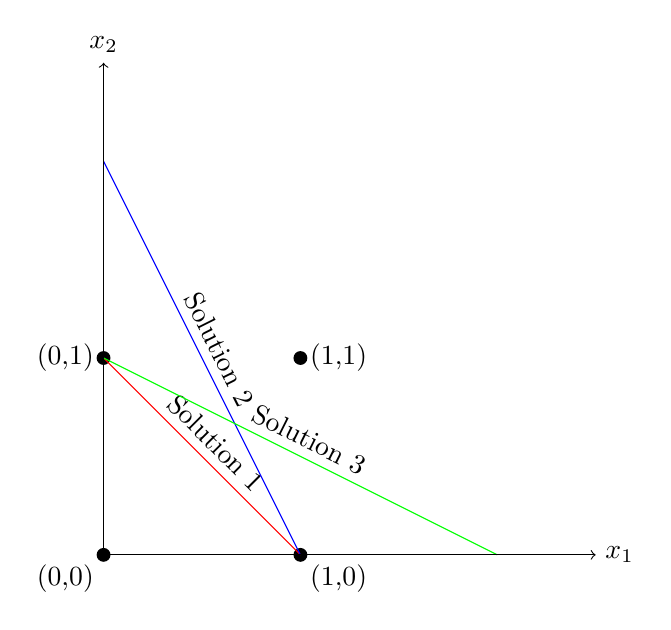
\begin{tikzpicture}[scale=2.5] % Adjust the scale for a larger plot
				      % Points
				      \fill (0,0) circle (1pt) node[below left] {(0,0)};
				      \fill (0,1) circle (1pt) node[left] {(0,1)};
				      \fill (1,0) circle (1pt) node[below right] {(1,0)};
				      \fill (1,1) circle (1pt) node[right] {(1,1)};

				      % Line with slope -1 and y-intercept 1
				      \draw[red] (0,1) -- (1, 0) node[midway, above,
					      sloped, black] {Solution 1};
				      \draw[blue] (0,2) -- (1, 0) node[midway, above,
					      sloped, black] {Solution 2};
				      \draw[green] (0,1) -- (2, 0) node[midway, above,
					      sloped, black] {Solution 3};

				      % Axes
				      \draw[->] (0, 0) -- (2.5,0) node[right] {$x_1$};
				      \draw[->] (0, 0) -- (0,2.5) node[above] {$x_2$};
			      \end{tikzpicture}
		      \end{center}

		      \textit{Note: Here learning rate $\alpha = 1$ and activation rule}
		      $ g(x) =
			      \begin{cases}
				      1 & \sum_i w_i x_i \geq 0 \\
				      0 & \text{otherwise}.
			      \end{cases} $
	      \end{tcolorbox}

\end{enumerate}

